\begin{figure}
\centering
\newcommand*{\testdir}[1]{{\scriptsize\texttt{#1}}}
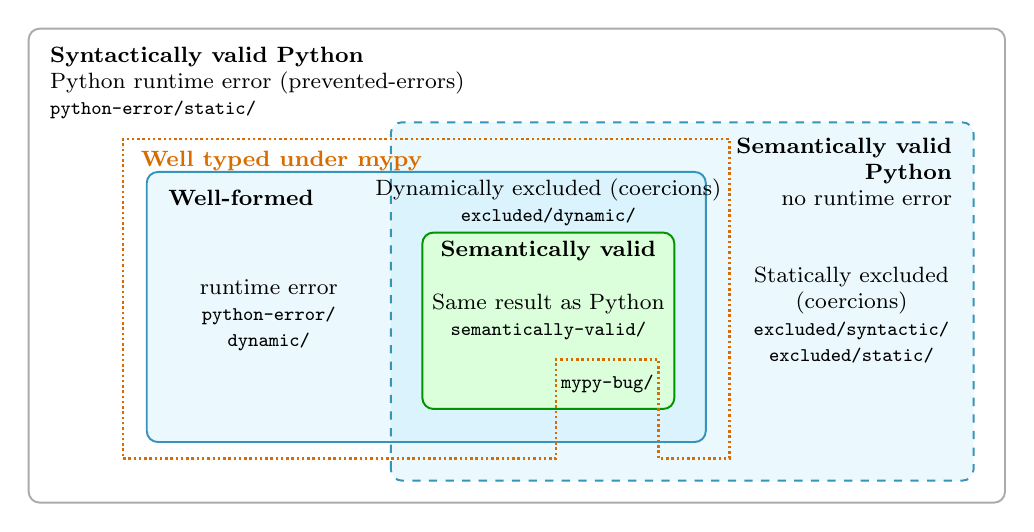
\begin{tikzpicture}[font=\footnotesize, rounded corners=4pt, yscale=0.7]
  \fill[cyan!60, fill opacity=0.13] (4.6,0.4) rectangle (12.0,6.9);
  \fill[cyan!60, fill opacity=0.13] (1.5,1.1) rectangle (8.6,6.0);
  \fill[green!14] (5.0,1.7) rectangle (8.2,4.9);
  \draw[black!33, line width=0.7pt] (0,0) rectangle (12.4,8.6);
  \draw[cyan!72!black, line width=0.7pt] (1.5,1.1) rectangle (8.6,6.0);
  \draw[dashed, cyan!72!black, line width=0.7pt] (4.6,0.4) rectangle (12.0,6.9);
  \draw[green!58!black, line width=0.7pt] (5.0,1.7) rectangle (8.2,4.9);
  \draw[densely dotted, orange!85!black, line width=0.9pt, sharp corners]
    (1.2,0.8) -- (6.7,0.8) -- (6.7,2.6) -- (8.0,2.6) -- (8.0,0.8) -- (8.9,0.8) -- (8.9,6.6) -- (1.2,6.6) -- cycle;
  \node[anchor=north west, align=left] at (0.15,8.45)
    {\textbf{Syntactically valid Python}\\Python runtime error (\figref{prevented-errors})\\\testdir{python-error/static/}};
  \node[anchor=north east, align=right] at (11.85,6.8)
    {\textbf{Semantically valid}\\\textbf{Python}\\no runtime error};
  \node[anchor=north west, text=orange!85!black] at (1.3,6.55) {\textbf{Well typed under mypy}};
  \node[anchor=north west] at (1.65,5.85) {\textbf{Well-formed \PurePy}};
  \node[align=center] at (10.45,3.4)
    {Statically excluded\\(\figref{coercions})\\\testdir{excluded/syntactic/}\\\testdir{excluded/static/}};
  \node[align=center] at (3.05,3.4) {\PurePy runtime error\\\testdir{python-error/}\\\testdir{dynamic/}};
  \node[align=center] at (6.6,5.45) {Dynamically excluded (\figref{coercions})\\\testdir{excluded/dynamic/}};
  \node[align=center] at (6.6,3.85)
    {\textbf{Semantically valid}\\\textbf{\PurePy}\\Same result as Python\\\testdir{semantically-valid/}};
  \node at (7.35,2.15) {\testdir{mypy-bug/}};
\end{tikzpicture}
\caption{Python programs and runs, classified by \PurePy, with test directories}
\label{fig:taxonomy}
\end{figure}
